\subsection{Lista de elementos}

  \paragraph{}La figura \ref{capturaListaElementos} muestra un ejemplo de
  listado de elementos. Como se puede observar, además aparecen elementos
  importantes que es necesario comentar:

  \begin{itemize}
   \item \textbf{Crear nuevos elementos}. Si el usuario dispone de los permisos
   necesarios aparecerá un icono, representado por una cruz verde junto con el
   texto \textit{Añadir nuevo}, que permitirá la adición de nuevos elementos.
   \item \textbf{Generar PDF}. Exporta el listado actual al formato PDF.
   \item \textbf{Búsqueda}. Se permite realizar búsquedas entre los elementos
   que componen la lista mostrada. La figura \ref{capturaBusquedaElementos}
   muestra un ejemplo de búsqueda de elementos.
   \begin{figure}[!ht]
    \begin{center}
      \fbox{
        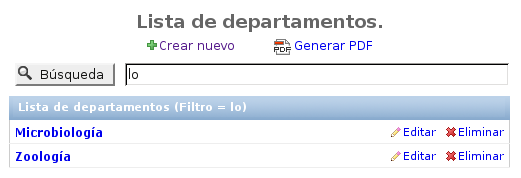
\includegraphics[scale=0.6]{12.Disenyo_Interfaz/12.3.Gestion_Informacion/12.3.1.Lista_Elementos/busqueda_elementos.png}
      }
      \caption{Captura de pantalla de una búsqueda de elementos.}
      \label{capturaBusquedaElementos}
    \end{center}
  \end{figure}
   \item \textbf{Ordenamiento}. Como cabecera de la lista de elementos,
   aparecerá el nombre del conjunto de elementos junto con una flecha indicando
   el tipo de ordenamiento: ascendente o descendente. Si se trata de elementos
   de tipo cadena su ordenamiento se realizará por orden alfabético, y si se
   trata de elementos numéricos de mayor a menor y viceversa.
   \item \textbf{Editar elemento}. Si el usuario dispone de los permisos
   necesarios aparecerá un icono, representado por un lápiz junto con el texto
   \textit{Editar}, que permitirá editar el elemento indicado.
   \item \textbf{Eliminar elemento}. Si el usuario dispone de los permisos
   necesarios aparecerá un icono, representado por una cruz roja girada 45
   grados con respecto a la vertical junto con el texto \textit{Eliminar}, que
   permitirá eliminar el elemento indicado, previa confirmación.
  \end{itemize}

  \begin{figure}[!ht]
    \begin{center}
      \fbox{
        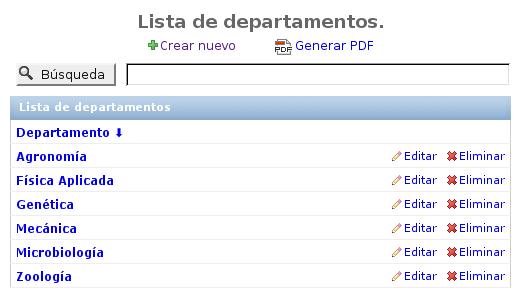
\includegraphics[scale=0.6]{12.Disenyo_Interfaz/12.3.Gestion_Informacion/12.3.1.Lista_Elementos/lista_elementos.png}
      }
      \caption{Captura de pantalla de un listado de elementos.}
      \label{capturaListaElementos}
    \end{center}
  \end{figure}